Training a CNN with millions of parameters on a small dataset could easily lead to horrible overfitting. But the idea of supervised pre-training on some huge image datasets could preventing this problem in certain degree. Compared to other randomly initialized strategies with certain distribution, supervised pre-training is to initialize the weights according to the model trained from a specific task. Indeed, initialization with pre-trained model has certain bias as there is no single dataset including all the invariance for natural images \cite{agrawal2014analyzing}, but this bias can be reduced as the pre-trained image dataset increases and the fine-tuning should be benefit from it.
\subsection{Pre-training and Fine-tuning}
We conduct several experiments on both architectures and use different training initialization strategies for both Food-256 and Food-101 datasets. The scratch models are initialized with Gaussian distribution for AlexNet and Xavier algorithm for GoogLeNet%, which automatically determines the scale of initialization based on the number of input and output neurons
 \cite{glorot2010understanding}. These two initializations are used for training the original models for the ImageNet task. The ft-last and fine-tuned models are initialized with the weights pre-trained from ImageNet dataset. For the ft-last model, we just re-train the fully connected layers while the whole network is fine-tuned for the fine-tune model.
\begin{table}[htbp]
  \centering
  \caption{Top-5 Accuracy in percent on fine-tuned, ft-last and scratch model for two architectures}
    \begin{tabular}{r|cc|cc}
    \toprule
          & \multicolumn{2}{c|}{AlexNet} & \multicolumn{2}{c}{GoogLeNet} \\    \midrule
     & Food-101   & Food-256   & Food-101   & Food-256 \\
    Fine-tune & \textbf{88.12} & \textbf{85.59} & \textbf{93.51} & \textbf{90.66} \\
    Ft-last &76.49	&79.26&	82.84	&83.77\\
    Scratch & 78.18 & 75.35 & 90.45 & 81.20 \\
    \bottomrule
    \end{tabular}%
  \label{tab:ft}%
\end{table}%


% Table generated by Excel2LaTeX from sheet 'Sheet1'
\begin{table}[htbp]
  \centering
  \caption{Accuracy compared to other method on Food-256 dataset in percent}
    \begin{tabular}{cC{3cm}cc}
    \toprule
     & fv+linear \cite{Kawano:2014} & GoogLeNet & AlexNet \\
     
    \midrule
    Top1  & 50.1& \textbf{70.13} & 63.82 \\
    Top5  & 74.4  & \textbf{90.66} & 85.59\\
    \bottomrule
    \end{tabular}%
  \label{tab:256}%
\end{table}%

% Table generated by Excel2LaTeX from sheet 'Sheet1'
\begin{table*}[htbp]
  \centering
  \caption{Top-1 accuracy compared to other methods on Food-101 dataset in percent}
    \begin{tabular}{c|C{3cm}C{3cm}cc}
    \toprule
          & RFDC\cite{bossard14} & MLDS($\approx$\cite{singh2012unsupervised}) & GoogLeNet & AlexNet \\
    \midrule
    Top1 accuracy & 50.76 & 42.63& \textbf{78.11 }& 66.40 \\
    \bottomrule
    \end{tabular}%
    \label{tab:101}
\end{table*}%
\begin{figure*}[htbp]
  \centering
  % Requires \usepackage{graphicx}
  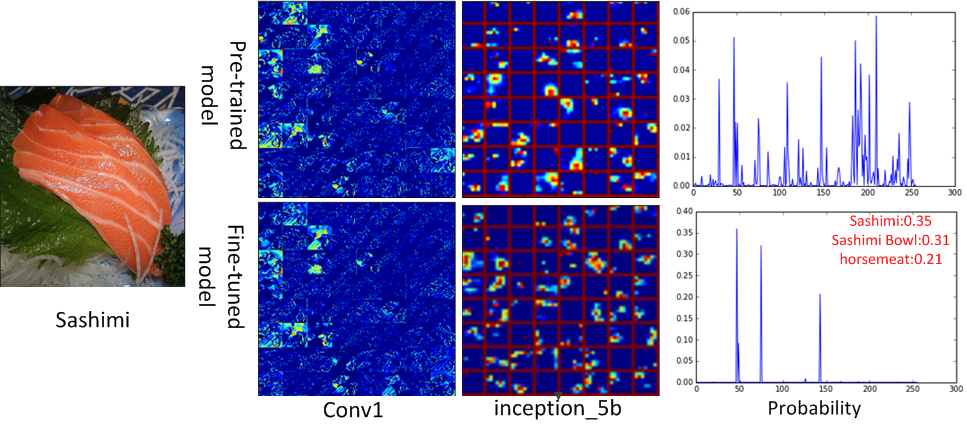
\includegraphics[scale=0.5]{fig/sashimi.png}\\
  \caption{Visualization of some feature maps of different GoogLeNet models in different layers for the same input image. 64 feature maps of each layer are shown. Conv1 is the first convolutional layer and Inception\_5b is the last convolutional layer. }
   \label{fig:sashimi}
\end{figure*}
From Table \ref{tab:ft} we can see that fine-tuning the whole network can improve the performance of the CNN for our task. Compared to other traditional computer vision methods (see Table \ref{tab:256} and \ref{tab:101}), GoogLeNet outperforms the other methods with large margins and we provide the state-of-the-art performance of these two food image datasets.

In Figure \ref{fig:sashimi} we visualize the feature maps of the pre-trained GoogLeNet model and fined-tuned GoogLeNet model with the same input image for some layers. We can see that the feature maps of the lower layer are similar as the lower level features are similar for most recognition tasks.
Then we can see that the feature maps in the high-level are different which leads to totally different recognition results.
Since only the last layer (auxiliary classifier) of the ft-last model is optimized, we can infer that the higher level features are more important which is consistent with our intuition. Also from Table \ref{tab:ft}, it is interesting to see that for the Food-101 task, the accuracy of  the scratch models outperforms the pre-trained models. Since Food-101 is a relatively large dataset with 750 images per class while Food-256 dataset is an imbalanced small one, this indicates that it is difficult to obtain a good deep CNN model while the data is insufficient.

From Table \ref{tab:ft} we can see that GoogLeNet always performances better than AlexNet on both datasets. This implies that the higher level features of GoogLeNet are more discriminative compared to AlexNet and this is due to the special architecture of its basic unit, Inception module. Table \ref{tab:cosg} and \ref{tab:cosa} show the weights' cosine similarity of each layer between the fine-tuned models and their pre-trained models. From the results we can see that the weights in the low layer are more similar which implies that these two architectures can learn the hierarchical features. As the low level features are similar for most of the tasks, the difference of the objects is determined by high-level ones which are the combination of these low level features. Also from Table \ref{tab:cosa}, we can observe that, the weights of the pre-trained and fine-tuned models are extremely similar in AlexNet . This can be caused by the size of receptive filed. Since ReLUs are used in both architectures, vanishing gradients do not exist. Rectified activation function is mathematically given by:
      \begin{equation}\label{relu}
        h = \max ({w^T}x,0) = \left\{ {\begin{array}{*{20}{c}}
{{w^T}x}&{{w^T}x > 0}\\
0&{else}
\end{array}} \right.
      \end{equation}

    The ReLU is inactivated when its input is below 0 and its partial derivative is 0 as well. Sparsity can improve the performance of the linear classifier on top, but on the other hand, sparse representations make the network more difficult to train as well as fine-tune. The derivative of the filter is $\frac{{\partial J}}{{\partial w}} = \frac{{\partial J}}{{\partial y}}\frac{{\partial y}}{{\partial w}} = \frac{{\partial J}}{{\partial y}}*x$ where $\frac{{\partial J}}{{\partial y}}$ denotes the partial derivative of the activation function, $y=w^Tx$ and $x$ denotes the inputs of the layer. The sparse input could lead to sparse filter derivative for back propagation which would eventually prevent the errors passing down effectively. Therefore, the filters of the fine-tuned AlexNet is extremely similar. Compared to large receptive field used in AlexNet, the inception module in GoogLeNet employs 2 additional $n\times n\_reduced$ convolutional layers before the $3\times 3$ and $5\times 5$ convolutional layers (see Figure \ref{incept}). Even though the original purpose of these two $1\times 1$ convolutional layer is for computational efficiency, these 2 convolutional layers tend to squeeze their sparse inputs and generate a dense outputs for the following layer. We can see from Table \ref{tab:sparse} that the sparsity of the $n\times n\_reduce$ layers are denser than other layers within the inception module. This makes the filters in the following layer more easily to be trained for transfer learning and generate efficient sparse representations.
  %\item The pooling strategy. In AlexNet, max pooling is applied to all the pooling layers between several convolution layers. During back propagation, the max pooling layer always passes the error to the place where it came from. Since it only came from one place of the receptive field, the back propagation error is sparse and keeps the most filters unchanged. In GoogLeNet, even though, there is a max pooling layer within every inception module, there are other 3 back propagation errors, from $5\times 5\_reduce$ and $3\times 3\_reduce$ that can parse dense back propagation errors to the previous inception module.


\begin{table*}[htbp]
  \centering
  \caption{Cosine similarity of the layers in inception modules between fine-tuned models and pre-trained model for GoogLeNet}
    \begin{tabular}{r|cccccc}
    \toprule
    \multicolumn{7}{c}{food256} \\
    \midrule
          & \multicolumn{1}{l}{1x1} & \multicolumn{1}{l}{3x3\_reduce} & \multicolumn{1}{l}{3x3} & \multicolumn{1}{l}{5x5\_reduce} & \multicolumn{1}{l}{5x5} & \multicolumn{1}{l}{pool\_proj } \\
    inception\_3a & 0.72  & 0.72  & 0.64  & 0.67  & 0.73  & 0.69 \\
    inception\_3b & 0.59  & 0.64  & 0.53  & 0.70  & 0.60  & 0.56 \\
    inception\_4a & 0.46  & 0.53  & 0.54  & 0.50  & 0.67  & 0.38 \\
    inception\_4b & 0.55  & 0.58  & 0.63  & 0.52  & 0.69  & 0.41 \\
    inception\_4c & 0.63  & 0.64  & 0.63  & 0.57  & 0.68  & 0.52 \\
    inception\_4d & 0.60  & 0.62  & 0.60  & 0.58  & 0.68  & 0.50 \\
    inception\_4e & 0.60  & 0.61  & 0.67  & 0.61  & 0.68  & 0.50 \\
    inception\_5a & 0.51  & 0.53  & 0.58  & 0.48  & 0.60  & 0.39 \\
    inception\_5b & 0.40  & 0.44  & 0.50  & 0.41  & 0.59  & 0.40 \\  \toprule
    \multicolumn{7}{c}{food101} \\ \midrule
          & \multicolumn{1}{l}{1x1 } & \multicolumn{1}{l}{3x3\_reduce} & \multicolumn{1}{l}{3x3} & \multicolumn{1}{l}{5x5\_reduce} & \multicolumn{1}{l}{5x5} & \multicolumn{1}{l}{pool\_proj } \\
    inception\_3a & 0.71  & 0.72  & 0.63  & 0.67  & 0.73  & 0.68 \\
    inception\_3b & 0.56  & 0.63  & 0.50  & 0.71  & 0.60  & 0.53 \\
    inception\_4a & 0.43  & 0.50  & 0.50  & 0.47  & 0.62  & 0.36 \\
    inception\_4b & 0.48  & 0.52  & 0.57  & 0.50  & 0.67  & 0.35 \\
    inception\_4c & 0.57  & 0.61  & 0.59  & 0.53  & 0.63  & 0.47 \\
    inception\_4d & 0.54  & 0.58  & 0.53  & 0.54  & 0.64  & 0.44 \\
    inception\_4e & 0.53  & 0.54  & 0.61  & 0.55  & 0.62  & 0.42 \\
    inception\_5a & 0.43  & 0.47  & 0.53  & 0.45  & 0.57  & 0.34 \\
    inception\_5b & 0.36  & 0.39  & 0.46  & 0.38  & 0.52  & 0.37 \\
    \bottomrule
    \end{tabular}%
  \label{tab:cosg}%
\end{table*}%


\begin{table*}[htbp]
  \centering
  \caption{Cosine similarity of the layers between fine-tuned models and pre-trained model for AlexNet}
    \begin{tabular}{r|ccccccc}
    \toprule
          & conv1 & conv2 & conv3 & conv4 & conv5 & fc6   & fc7 \\
    \midrule
    food256 & 0.997 & 0.987 & 0.976 & 0.976 & 0.978 & 0.936 & 0.923 \\
    food101 & 0.996 & 0.984 & 0.963 & 0.960 & 0.963 & 0.925 & 0.933 \\
    \bottomrule
    \end{tabular}%
  \label{tab:cosa}%
\end{table*}%

% Table generated by Excel2LaTeX from sheet 'google'
\begin{table*}[htbp]
  \centering
  \caption{Sparsity of the output for each unit in GoogLeNet inception module for training data from Food101 in percent}
    \begin{tabular}{r|cccccc}
    \toprule
          & 1x1  & 3x3\_reduce & 3x3  & 5x5\_reduce & 5x5  & pool\_proj  \\
    \midrule
    inception\_3a & $69.3\pm 1.3$  & $69.6 \pm 1.1$  & $80.0\pm  1.0$& $64.1\pm  2.2$& $75.8\pm  1.6$& $76.2\pm 5.4$\\
    inception\_3b & $92.8 \pm 0.9$&$ 76.5 \pm 0.9$& $94.7\pm 0.9 $&$ 71.6 \pm 2.3 $&$ 94.4\pm 0.5 $&$ 94.7 \pm 1.6$\\
    inception\_4a & $90.9 \pm 0.9$& $70.0\pm 1.2 $& $93.8\pm 1.1 $& $63.3\pm 4.0 $& $91.9\pm 1.8 $& $95.1\pm 2.0$\\
    inception\_4b & $71.9 \pm 1.6$& $67.5\pm 1.2$ & $75.4\pm  1.0$& $58.5 \pm 2.6$& $78.9\pm  1.6$& $85.6\pm 3.6$\\
    inception\_4c & $75.1 \pm 2.4$& $72.6 \pm 1.3$& $81.0\pm 2.0$ & $66.3\pm 6.1 $& $79.7 \pm 3.6$& $88.1\pm 3.3$\\
    inception\_4d & $87.3 \pm 2.7$& $78.0 \pm 2.2$& $88.0\pm 1.6$& $67.9\pm 3.1 $& $88.9\pm 2.8 $& $93.0\pm 2.2$\\
    inception\_4e & $91.8\pm  1.1$& $62.3\pm 2.2 $& $91.0\pm 2.5 $& $49.5 \pm 3.7$& $94.0 \pm 1.0$& $92.3\pm 1.5$\\
    inception\_5a & $78.7 \pm 1.6$& $66.5\pm  1.7$& $82.3\pm 2.6 $& $59.9\pm 3.2 $& $86.4\pm 2.3 $& $87.1\pm 2.6$\\
    inception\_5b & $88.2\pm 2.3 $& $86.8 \pm 1.6$&$ 83.3\pm 4.4$ & $84.0\pm 3.1 $& $81.4\pm 5.3$  & $94.7\pm 1.5$\\
    \bottomrule
    \end{tabular}%
  \label{tab:sparse}%
\end{table*}%

The unique structure of the Inception module guarantees that the sparse outputs from previous layer can be squeezed with the $1\times 1$ convolutional layers and feed to convolutional layers with bigger receptive field to generate sparser representation. The squeeze action promises the back propagation error can be transferred more efficiently and makes the whole network more flexible to fit different recogntion tasks.

\subsection{Learning across the datasets}
From the previous experiments we can see that pre-training on the ImageNet dataset can improve the performance of the deep convolutional neural network on our specific area. In this part, we will discuss the generalization ability within the food recognition problem.  Zhou et al. trained AlexNet for Scene Recognition across two datasets with identical categories \cite{NIPS2014_Zhou}. But for more complex situation, such as two similar datasets with a little overlapped categories, we are very interested in exploring whether deep CNN can still successfully handle. Therefore, we conduct the following experiment to stimulate a more challenging real world problem: transferring the knowledge from the fine-tuned Food-101 model to a target set, Food-256 dataset. To make the experiment more practical, we limit the number of samples per category from Food-256 for training, because if we want to build a our own model using deep CNN for a specific task, the resource is always limited and it is exhausted to collect hundreds of labeled images for each category.

The Food-101 and Food-256 datasets share about 46 categories of food even though the images in the same category may vary across these two datasets. The types of food in Food-101 are mainly western style while most types of food in Food-256 are typical Asian foods. We compare the top-5 accuracy trained from different size of subset for Food-256 on different pre-trained model and the results are shown in Table \ref{tab:cross}.
%The ImageNet columns denote  the pre-trained model trained only on ImageNet images and the Food101\_ft columns denote the pre-trained model trained on ImageNet images and then fine-tuned on Food-101.
The ImageNet columns denote using the model pre-trained from ImageNet dataset as the pre-trained model and Food101\_ft columns denote using the fine-tuned Food-101 model (the same one in Table \ref{tab:ft}) as the pre-trained model.

From the result of Table \ref{tab:cross} we can see that, with this further transfer learning, both CNNs can achieve around 95\% of the accuracy trained on full dataset while just utilizing about half of them (50 per class, 12800 of 25361 images). This indicates that when there is not enough labeled data, with its strong generalization ability, deep CNN trained from general task can still achieve satisfying result and perform even better when an additional relevant dataset is involved. This encouraging result may attract more people to use deep CNN for their specific task and continue to explore the potential of the existing architecture as well as designing new ones.

\begin{table*}[htbp]
  \centering
  \caption{Top5 Accuracy for transferring from Food101 to subset of Food256 in percent}
    \begin{tabular}{c|cc|cc}
    \toprule
          & \multicolumn{2}{c|}{AlexNet} & \multicolumn{2}{c}{GoogLeNet} \\
    \midrule
    instances per class & ImageNet  & Food101\_ft    &  ImageNet  & Food101\_ft \\ \midrule
    20    & 68.80  & {75.12} & 74.54 & {77.77} \\
    30    & 73.15 & {77.02} & 79.21 & {81.06} \\
    40    & 76.04 & {80.23} & 81.76 & {83.52} \\
    50    & 78.90  & {81.66} & 84.22 & {85.84} \\
    all    & 85.59 &  {87.21} & {90.66 }&   {90.65}     \\
    \bottomrule
    \end{tabular}%
  \label{tab:cross}%
\end{table*}%

